\documentclass[a4paper]{article}

\setcounter{secnumdepth}{0}

%Metadata
\title{Kuwaiba Open Inventory user's Manual}
\author{Neotropic SAS}
\date{27.07.2016}

%Imports
\usepackage{graphicx}
\usepackage[utf8]{inputenc}
\usepackage{booktabs}
\usepackage[margin=3cm]{geometry}
\usepackage{color}
\usepackage{framed}
\usepackage{verbatimbox}
\usepackage[toc,page]{appendix}
\usepackage{nameref}

%\usepackage{hyperref}

%Modify some defaults
\setlength{\parindent}{0pt} %don't indent new paragraphs

\begin{document}
	\maketitle
	\pagenumbering{gobble}
	
	
	
	\begin{figure}[b]
		\centering System Version \textbf{1.0}
			
		Visit \textbf{kuwaiba.org} for documentation, latest updates and upcoming events
	\end{figure}
	
	
	\newpage
	
	\tableofcontents

	\newpage
	\section{Document History}
		\begin{table}[h!]
			\centering
			\begin{tabular}{l||p{10cm}} %Each letter tells the parser what alignment should have every column
				\toprule
				\textbf{Date} & \textbf{Comments}  \\
				\midrule
				September 28th 2010 & First issue shipped with version 0.1.1\\
				\midrule
				November 26th 2010 & Update to cover the new features in 0.2 \\
				\midrule
				December 26th 2010 & Update to cover the new features in 0.2.1 \\
				\midrule
				January 18 th 2001 & Changes in version 0.3 alpha \\
				\midrule
				February 3 rd 2011 & Changes in version 0.3 beta \\
				\midrule
				March 13 th	2011 & Changes in version 0.3 beta 2 \\
				\midrule
				May 16th 2011 & Changes in version 0.3 stable (the clear button in the graphical query editor \\
				\midrule
				May 23rd 2012 & Adapted to version 0.4 \\
				\midrule
				October 23rd 2012 & Adapted to version 0.5 \\
				\midrule
				June 4 th 2013 & Added documentation	for Pools module \\
				\midrule
				June 12 th 2013 & Added documentation for Data model Manager module and some other minor changes\\
				\midrule
				January 19 th 2015 & Adapted manual for version 0.7 \\
				\midrule
				November 6 th 2015 & Added documentation about bulk upload, software asset management and detailed physical connections \\
				\midrule
				July 27th 2016 & Adapted to Kuwaiba version 1.0. LaTeX is now used instead of LibreOffice to create the documentation. \\
				\bottomrule
			\end{tabular}	
				
		\end{table}
	\newpage
	\section{License}
		\begin{table}[ht]
			\centering
			\begin{tabular}{cp{10cm}}
				
				
\includegraphics[]{img/cc_license_logo.jpg} & This document is published under the terms of a license Creative Commons by-nc-sa. You can find details about it at\linebreak
				\textbf{http://creativecommons.org/licenses/by-nc-sa/2.0/ } \\

				
\includegraphics[width=2cm]{img/osi_logo.jpg} & Kuwaiba Server and Client are licensed under EPL v1 and GPL v2. You can find the whole text of this licenses at \linebreak
				\textbf{http://www.eclipse.org/legal/epl-v10.html} \linebreak
				\textbf{http://www.gnu.org/licenses/old-licenses/gpl-2.0.html} \\
			\end{tabular}
		\end{table}
		\paragraph{Disclaimer} \hspace{0pt}
		\begin{itemize}
			\item Netbeans and Java are registered trademarks of Oracle and/or its affiliates. Other names may be trademarks of their respective owners. The Kuwaiba project is not endorsed to any of them.
			
			\item This document is provided “as is”, with no warranty at all. Install the software and follow the instructions included at your own risk.
			
			\item Kuwaiba uses third-party components with compatible open source licenses (LGPL, BSD-like, etc). You can find a complete list at the project's web page.
		\end{itemize}
	
	\newpage
	\pagenumbering{arabic}
	\section{Introduction}
	Kuwaiba sees an inventory system as a living entity, not growing only in terms of size, but also in structure and intelligence. The main reason is that business requirements change constantly and therefore, the application must ready to respond to new scenarios. One of the key concepts that can help you unlock the potential of Kuwaiba is the \textbf{data model}. It provides a simplified representation of the network and the business from an operational point of view. It can be seen as the skeleton that supports the application, but a skeleton from which you can add, remove and change elements as you go. Later in this document you will be able to see what tools you can use to manage it. For now, just keep in mind that the better you design your data model and the more you get to know it, the more you will take advantage of the application.\newline
	
	Having said that, you will find four types of resources in a typical data model:
	\begin{itemize}
		\item \textbf{Physical:} Equipment, pipes, cables, fiber optics, facilities, parts and in general every physical asset from a port to a building. 
		\item \textbf{Logical:} These are all the resources related to non-tangible technology assets. In this group fits timeslots, virtual circuits, VLANs, disk space, available bandwidth, etc.
		\item \textbf{Other Non-physical:} mostly software-related assets, such as licenses or virtual machines.
		\item \textbf{Administrative:} These are all those related to administrative tasks, human resources or commercial management. Customers, their services, SLAs (and related parameters like availability or throughput), sales and technical staff assigned to those services, vendors and states belong to this category.
	\end{itemize}
	The Kuwaiba desktop client is a set of views (trees, topologies, editors) that allow to put together these elements based on business rules and  user-defined models. Kuwaiba extends the concept of \textbf{CMDB} (Configuration Management Database, a place where you store objects that can hold configuration information or be subject to configuration themselves -so called Configuration Items- and their relationships)  and enables you to perform network design tasks, support capacity management and provisioning workflows and assist field and customer service teams to improve response times.\newline
	
	Kuwaiba helps you model your network according to your needs, no matter if you're an ISP, a carrier or just a guy with a large (or small!) IT infrastructure to manage. It's open source, under active development and new models are added every release. You can contribute to the project by providing technical insight on a particular technology, testing, translating or just sending your feedback through forums\footnote{Forums https://sourceforge.net/p/kuwaiba/discussion/} and mailing lists\footnote{mailing lists https://sourceforge.net/p/kuwaiba/mailman/}.
	
	\newpage
	\section{Connection to the Server}
	The first thing you will see when opening the client is the window in the figure~\ref{fig:auth_window}. The default user and password are \textbf{admin/kuwaiba}.
	 
	\begin{figure}[h!]
		\centering
		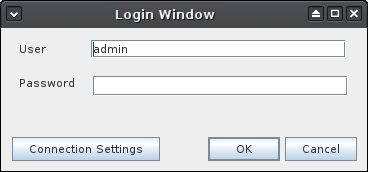
\includegraphics[width=0.5\linewidth]{img/auth_window.png}
		\caption{Authentication window}
		\label{fig:auth_window}
	\end{figure}
	The default connection settings should be enough if the server is running on the same computer the client is. If that's not the case, open the Connection Settings window (figure~\ref{fig:connection_settings}).
	\begin{figure}[h!]
		\centering
		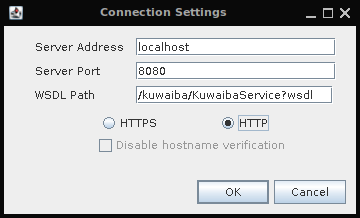
\includegraphics[width=0.5\linewidth]{img/connection_settings.png}
		\caption{Connection Settings window}
		\label{fig:connection_settings}
	\end{figure}
	\begin{itemize}
		\item \textbf{Server Address} Refers to the server IP address or canonical name.
		\item \textbf{Server Port} is the port Glassfish (the application server) is listening to.
		\item \textbf{WSDL Path} is the path within the application server the web service interface definition can be found. Usually this value should remain unchanged.
		\item Protocol is the transport protocol to be used. By default is HTTP, but is highly advisable to request your administrator to setup a secure connection, otherwise your credentials will be transmitted in plain text over the network. 
	\end{itemize}
	Except for the password, the last successful settings will be saved upon clicking OK.
	\begin{framed} {\large \textbf{Important}} \\
		If you are unsure if the server is reachable from your location, open a browser and type the address: \textbf{http://[server\_address]:[server\_port]/[wsdl\_location]}\\
		
		You should see a large XML document.
	\end{framed}
	\begin{framed} {\large \textbf{Troubleshooting}}
		\begin{itemize}
			\item For a \textbf{\textcolor{red}{Can't contact backend}} error, check the Administrator's Manual Troubleshooting section.
			\item If you get a \textbf{\textcolor{red}{Connection refused}} error, check the connection settings and verify that the server is reachable and there isn't a firewall blocking the traffic to it.
		\end{itemize}
	\end{framed} 
	Once you are logged in, you will see only the dashboard page and a toolbar (figure~\ref{fig:main_toolbar}).\\
	\begin{figure}[h!]
		\centering
		
\includegraphics[width=0.7\linewidth]{img/main_toolbar.png}
		\caption{Main toolbar}
		\label{fig:main_toolbar}
	\end{figure}
	
	The toolbar contains the most frequently used tools. Here is an overview of what cab you do with them:
	\begin{table}[h!]
		\centering
		\begin{tabular}{cl}
			
\includegraphics[width=0.5cm]{img/icon_query_manager.png} & Search objects with the Query Manager\\
			\midrule
			
\includegraphics[width=0.5cm]{img/icon_refresh_component.png} & Refresh the current view\\
			\midrule
			
\includegraphics[width=0.5cm]{img/icon_refresh_cache.png} & Refresh local cache\\
			\midrule
			
\includegraphics[width=0.5cm]{img/icon_object_view.png} & Default view for an object. Also, the rack view for rack objects\\
			\midrule
			
\includegraphics[width=0.5cm]{img/icon_task_manager.png} & Create automation tasks (beta version)\\
			\midrule
			
\includegraphics[width=0.5cm]{img/icon_audit_trail.png} & See the changes made to inventory and application objects\\
			\midrule
			
\includegraphics[width=0.5cm]{img/icon_user_manager.png} & Manage users and groups\\
			\midrule
			
\includegraphics[width=0.5cm]{img/icon_data_model_manager.png} & Change the data model\\
			\midrule
			
\includegraphics[width=0.5cm]{img/icon_containment_manager.png} & Manage how objects can be created inside others\\
			\midrule
			
\includegraphics[width=0.5cm]{img/icon_list_type_manager.png} & Create new list types\\
			\midrule
			
\includegraphics[width=0.5cm]{img/icon_topology_designer.png} & Freely design network topologies\\
			\midrule
			
\includegraphics[width=0.5cm]{img/icon_navigation_tree.png} & Main tree used to explore physical assets\\
			\midrule
			
\includegraphics[width=0.5cm]{img/icon_pools_manager.png} & Create and manage objects that don't fit in the navigation tree\\
			\midrule
			
\includegraphics[width=0.5cm]{img/icon_service_manager.png} & Manage client, services and resources associated to them\\
		\end{tabular}	
		\caption{Toolbar items}
	\end{table}
	
	\newpage
	\section{Data Model Manager}
		One of the key features of Kuwaiba is that it is completely object-oriented\footnote{Object-oriented Programming https://en.wikipedia.org/wiki/Object-oriented\_programming}. It means that every business (Router, City, Port) and application (users, types) element is represented by an \textbf{Object} in the application and these objects are in turn product of an reality abstraction called \textbf{Class}. Likewise, every attribute is a \textbf{Field} in a class. The set of classes, attributes and relationships between them is called data model. There's a default data model, but you can customize it depending on your needs by adding, removing and modifying classes. To achieve this, use the Data Model Manager module (figure~\ref{fig:data_model_manager}).
		\begin{figure}[h!]
			\centering
			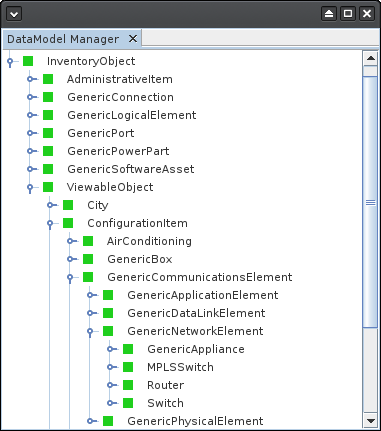
\includegraphics[width=0.4\linewidth]{img/data_model_manager.png}
			\caption{Part of the data model tree}
			\label{fig:data_model_manager}
		\end{figure}
		The data model is represented as a tree because it's a hierarchical structure. Technically, it's a class hierarchy\footnote{Class Hierarchy https://en.wikipedia.org/wiki/Class\_hierarchy}. The top of the hierarchy (\textbf{InventoryObject}) is the most general type of element in the data model and its subclasses represent all the possible elements that will be treated as inventory assets. As you dig deeper into the tree, the classes become more and more specialized and each level inherits the attributes of the parent classes. This kind of structure has two purposes: First, it helps you to organize your classes based on what characteristics they have in common. Secondly, as you will see later in this manual, you can apply operations over top level classes, and they will be propagated to all subclasses. Another root of the data model tree is \textbf{GenericObjectList}, and its subclasses are all possible list types (see more details on the subject in the chapter \textbf{\nameref{sec:list_type_manager}}).\newline
		
		\begin{framed} {\large \textbf{Important}} \\
				The \textbf{Properties} window allows you to modify the attributes of a selected object in a tree, list or view. If not already open, it's available from the Windows $\rightarrow$ Properties menu.
		\end{framed}
		The properties of a class can be edited by using the \textbf{Properties} window, selecting the class from the tree (see figure~\ref{fig:properties_class_node}). 
		\begin{figure}[h!]
			\centering
			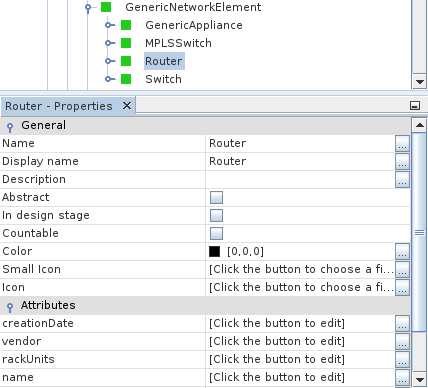
\includegraphics[width=0.5\linewidth]{img/properties_class_node.png}
			\caption{Properties of class \textbf{Router}}
			\label{fig:properties_class_node}
		\end{figure}
	\newpage
	\section{List Type Manager} \label{sec:list_type_manager}
\end{document}